\chapter{System Architecture}
\label{chap:architecture}

This chapter describes the overall architecture of the {\name} system, its components, and the design principles that guide its implementation.

\section{System Architecture Overview}
\label{sec:architecture_overview}

The {\name} system follows a multi-tier architecture designed to handle the complex process of web structure analysis and clustering. The architecture comprises four distinct layers: Frontend, API, Core Processing, and Data Storage.

\begin{figure}[h]
\centering
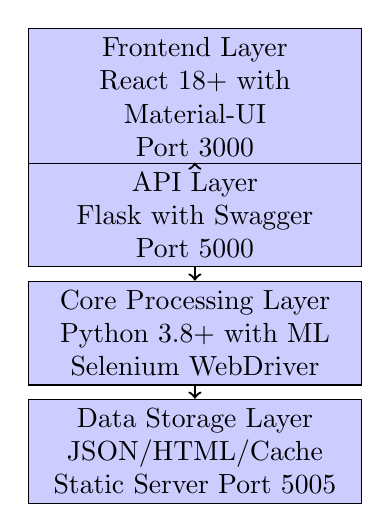
\begin{tikzpicture}[
    box/.style={rectangle, draw, fill=blue!20, text width=4cm, text centered, minimum height=1.2cm},
    arrow/.style={->, thick}
]
    \node[box] (frontend) at (0,4) {Frontend Layer\\React 18+ with Material-UI\\Port 3000};
    \node[box] (api) at (0,2.5) {API Layer\\Flask with Swagger\\Port 5000};
    \node[box] (processing) at (0,1) {Core Processing Layer\\Python 3.8+ with ML\\Selenium WebDriver};
    \node[box] (storage) at (0,-0.5) {Data Storage Layer\\JSON/HTML/Cache\\Static Server Port 5005};
    
    \draw[arrow] (frontend) -- (api);
    \draw[arrow] (api) -- (processing);
    \draw[arrow] (processing) -- (storage);
\end{tikzpicture}
\caption{{\name} System Architecture}
\label{fig:system_architecture}
\end{figure}

\subsection{Design Principles}

The system architecture is guided by several key design principles:

\begin{itemize}
\item \textbf{Modularity.} Each layer has clearly defined responsibilities and interfaces.
\item \textbf{Scalability.} The system can handle increasing loads through caching and optimization.
\item \textbf{Extensibility.} New clustering algorithms and analysis methods can be easily integrated.
\item \textbf{Usability.} The frontend provides an intuitive interface for both technical and non-technical users.
\end{itemize}

\section{Component Description}
\label{sec:component_description}

\subsection{Frontend Layer}

The frontend layer, implemented using React 18+ and Material-UI, provides the user interface for system interaction. The main component is URLChipForm.js, which implements a tabbed interface with the following sections:

\begin{itemize}
\item \textbf{Home Tab.} Handles URL input, validation, and processing configuration with support for bulk URL processing. Features include multi-URL paste functionality, domain-based grouping, and level selection (1-10 levels supported in the interface).
\item \textbf{Clusters Tab.} Displays clustering results with interactive color-coded representations, collapsible sections, and PDF export functionality using html2pdf.js.
\item \textbf{Experiments Tab.} Provides interface for batch processing, automated test case generation, and experimental result analysis with real-time progress tracking.
\item \textbf{Results Tab.} Shows archived experiment results and performance metrics with detailed timing logs and cache efficiency statistics.
\item \textbf{Config Tab.} Allows configuration of experimental parameters including URL combinations, DOM levels, and processing modes.
\end{itemize}

The interface supports both dark and light themes, includes a fixed navigation bar, GitHub integration link, and provides detailed error handling with user-friendly notifications.

\section{User Interface Design}
\label{sec:user_interface}

The {\name} system provides an intuitive web-based interface that guides users through the complete web structure analysis workflow. The interface design emphasizes usability while providing access to advanced features for researchers and practitioners.

\subsection{Main Interface Overview}

The primary interface features a tabbed navigation system that organizes functionality into logical sections:

\begin{figure}[h]
\centering
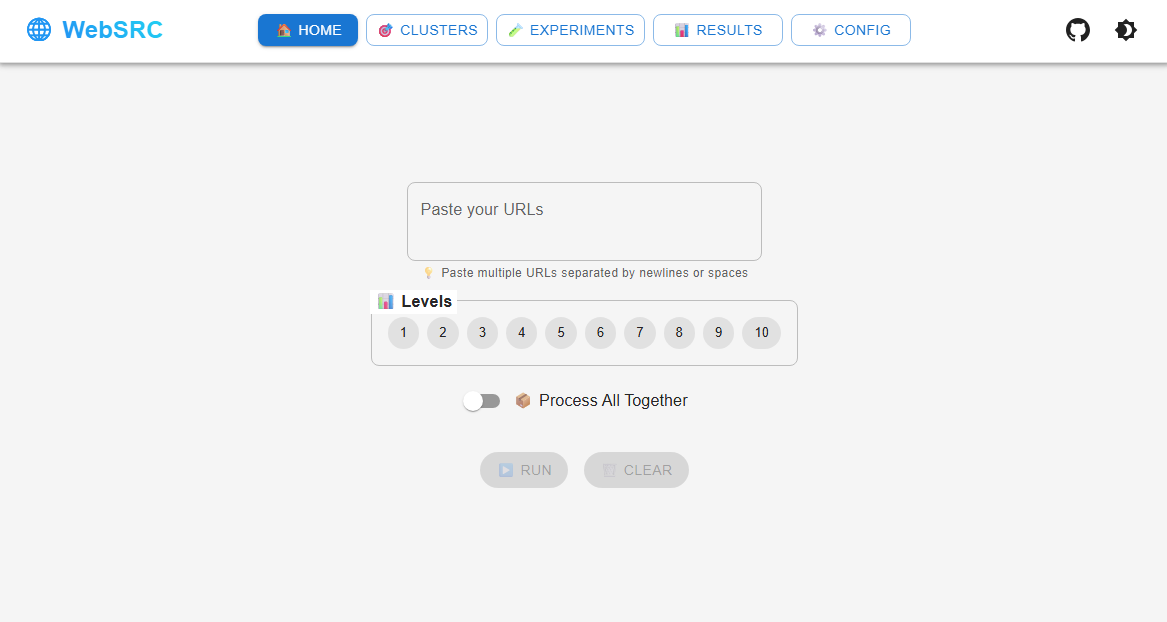
\includegraphics[width=\textwidth]{ui_main_interface.png}
\caption{Main Interface with Navigation Tabs and Theme Toggle}
\label{fig:ui_main_interface}
\end{figure}

\subsection{Home Tab - URL Processing Configuration}

The Home tab provides the primary interface for configuring and executing web structure analysis:

\begin{figure}[h]
\centering
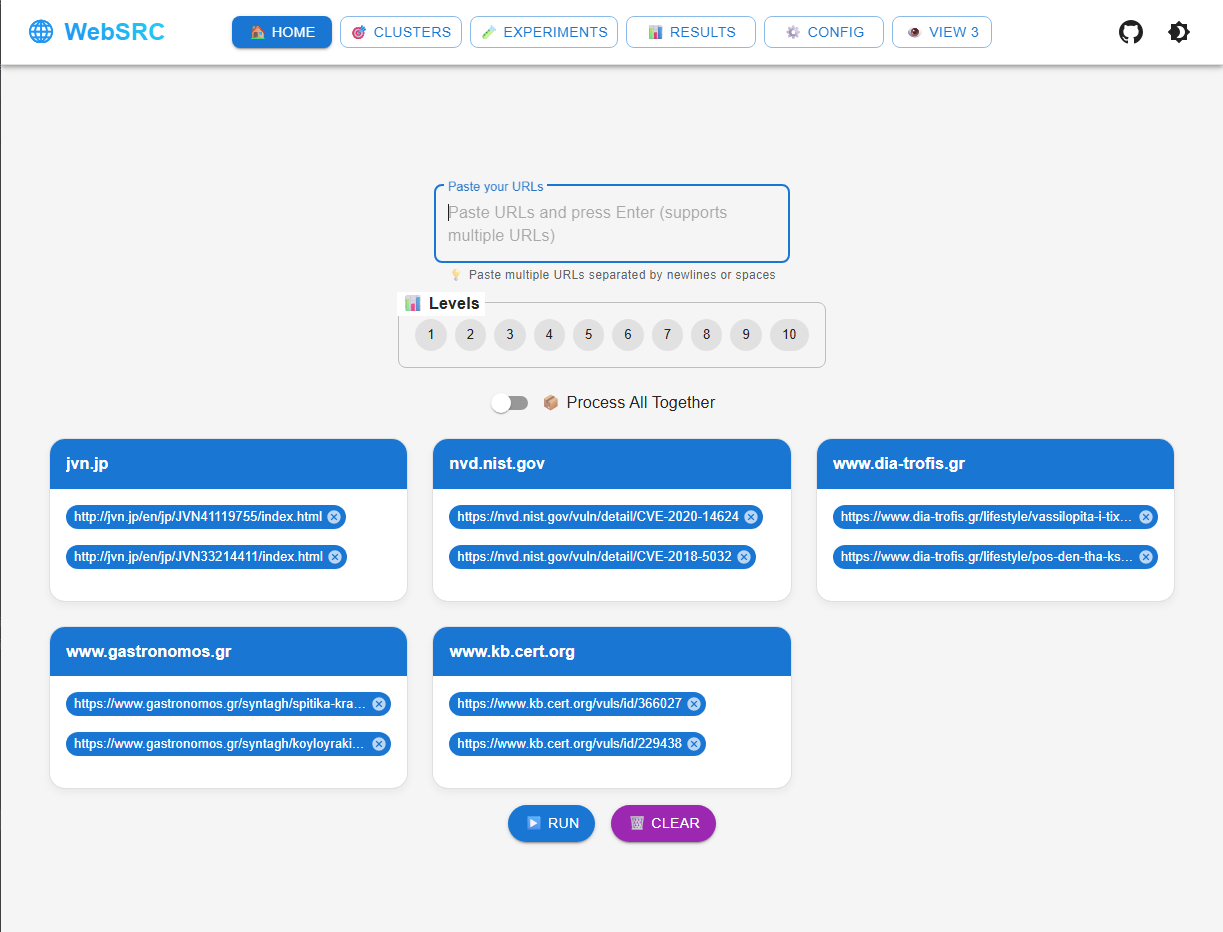
\includegraphics[width=\textwidth]{ui_home_tab.png}
\caption{Home Tab: URL Input and Configuration}
\label{fig:ui_home_tab}
\end{figure}

Key features include:
\begin{itemize}
\item \textbf{URL Input Field}: Multi-line text area supporting bulk URL entry with automatic parsing
\item \textbf{Level Selection}: Interactive chips for selecting DOM analysis depths (1-10 levels)
\item \textbf{Processing Mode}: Toggle between Mode 0 (All Together) and Mode 1 (Domain-based)
\item \textbf{Domain Grouping}: Automatic organization of URLs by domain in expandable cards
\end{itemize}

\begin{figure}[h]
\centering
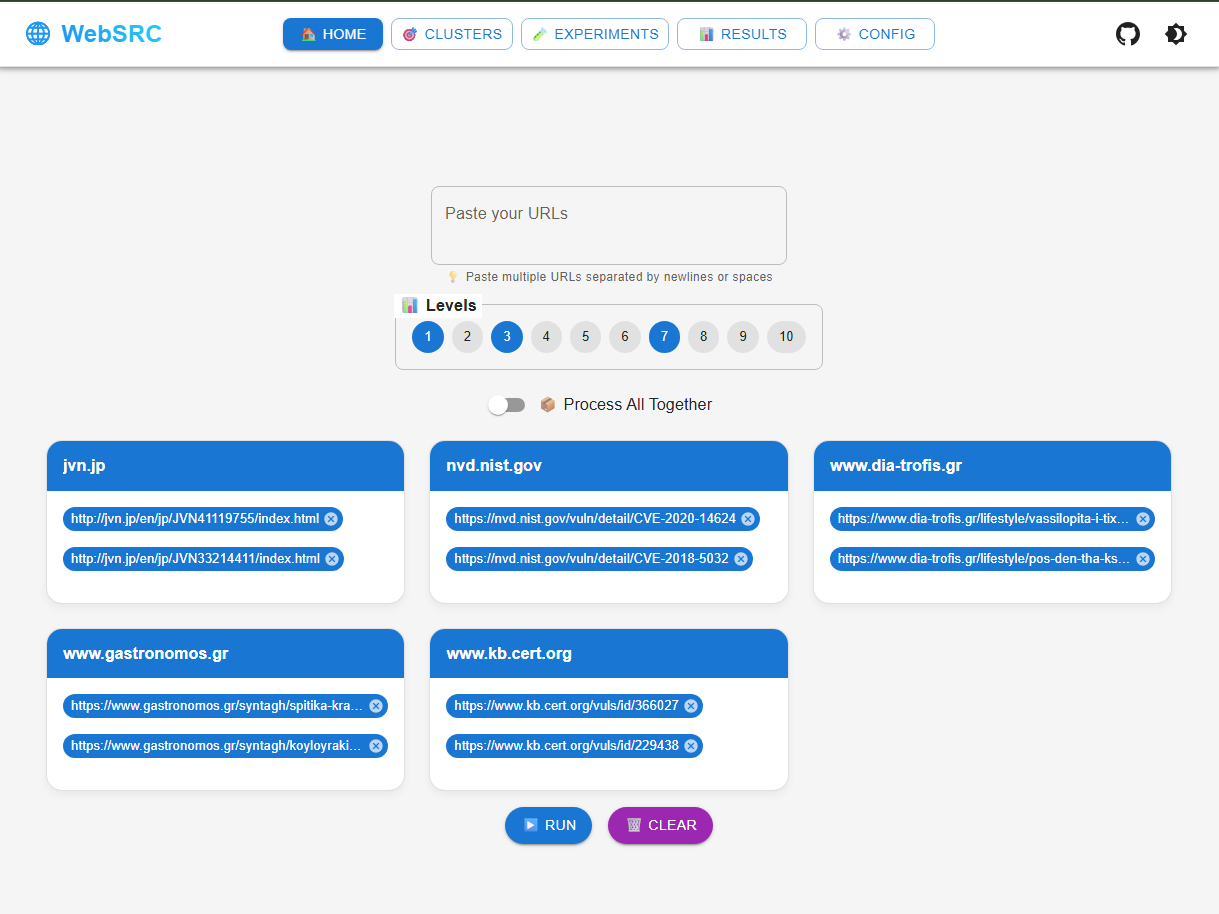
\includegraphics[width=\textwidth]{ui_level_selection.png}
\caption{DOM Level Selection Interface with Interactive Chips}
\label{fig:ui_level_selection}
\end{figure}

\begin{figure}[h]
\centering
\includegraphics[width=\textwidth]{ui_domain_grouping.png}
\caption{Domain-based URL Grouping with Expandable Cards}
\label{fig:ui_domain_grouping}
\end{figure}

\subsection{Clusters Tab - Results Visualization}

The Clusters tab displays clustering results with interactive visualizations:

\begin{figure}[h]
\centering
\includegraphics[width=\textwidth]{ui_clusters_tab.png}
\caption{Clusters Tab: Color-coded Clustering Results}
\label{fig:ui_clusters_tab}
\end{figure}

\begin{figure}[h]
\centering
\includegraphics[width=\textwidth]{ui_cluster_visualization.png}
\caption{Individual Cluster Visualization with Color Coding}
\label{fig:ui_cluster_visualization}
\end{figure}

Features include:
\begin{itemize}
\item \textbf{Level-based Organization}: Results grouped by DOM analysis level
\item \textbf{Color-coded Elements}: Visual representation of cluster assignments
\item \textbf{Collapsible Sections}: Expandable views for detailed examination
\item \textbf{PDF Export}: One-click export functionality using html2pdf.js
\end{itemize}

\subsection{Experiments Tab - Batch Processing}

The Experiments tab provides advanced functionality for research and batch analysis:

\begin{figure}[h]
\centering
\includegraphics[width=\textwidth]{ui_experiments_tab.png}
\caption{Experiments Tab: Test Case Management and Execution}
\label{fig:ui_experiments_tab}
\end{figure}

\begin{figure}[h]
\centering
\includegraphics[width=\textwidth]{ui_experiment_results.png}
\caption{Experiment Results with Performance Metrics}
\label{fig:ui_experiment_results}
\end{figure}

\subsection{Results Tab - Historical Data}

The Results tab provides access to archived experiment data:

\begin{figure}[h]
\centering
\includegraphics[width=\textwidth]{ui_results_archive.png}
\caption{Results Archive with Timing Logs and Cache Statistics}
\label{fig:ui_results_archive}
\end{figure}

\subsection{Configuration Tab - Advanced Settings}

The Config tab allows fine-tuning of experimental parameters:

\begin{figure}[h]
\centering
\includegraphics[width=\textwidth]{ui_config_tab.png}
\caption{Configuration Tab: Custom Experiment Parameters}
\label{fig:ui_config_tab}
\end{figure}

\subsection{Dark Mode Interface}

The system supports both light and dark themes for improved user experience:

\begin{figure}[h]
\centering
\includegraphics[width=\textwidth]{ui_dark_mode.png}
\caption{Dark Mode Interface with Theme Toggle}
\label{fig:ui_dark_mode}
\end{figure}

\subsection{API Layer}

The Flask-based API layer serves as the communication bridge between the frontend and core processing components. Primary endpoints include:

\begin{itemize}
\item \texttt{POST /process-urls}: Main URL processing endpoint with multi-level analysis support
\item \texttt{POST /process-clusters}: Cluster data processing and visualization generation
\item \texttt{POST /site-similarity}: Site similarity analysis using cosine similarity
\item \texttt{GET /cache/stats}: Cache performance statistics and efficiency metrics
\item \texttt{GET /experiments/test-cases}: Experimental framework endpoints for research evaluation
\end{itemize}

\subsection{Core Processing Layer}

The core processing layer implements the main algorithms and data processing logic:

\begin{itemize}
\item \textbf{DataCollector.} Handles web scraping and DOM structure extraction using Selenium WebDriver with comprehensive error handling and timing metrics.
\item \textbf{Clustering Engine.} Implements HDBSCAN-based clustering with DBCV validation, parameter optimization, and intelligent outlier reassignment.
\item \textbf{Cache Manager.} Provides intelligent caching with dual-layer architecture supporting both complete and partial cache strategies.
\item \textbf{Similarity Analyzer.} Computes cosine similarity between website structures and generates comparative analysis reports.
\end{itemize}

\subsection{Data Storage Layer}

The data storage layer manages all persistent data and generated content:

\begin{itemize}
\item \textbf{Structured Data Storage.} JSON files containing DOM elements, CSS properties, and clustering results.
\item \textbf{Visualization Files.} HTML files with color-coded clustering visualizations served by static server.
\item \textbf{Cache System.} Dual-layer caching with metadata tracking and automatic expiration management.
\item \textbf{Experiment Archive.} Comprehensive storage of experimental results and performance metrics.
\end{itemize}

\section{Technology Stack}
\label{sec:technology_stack}

\subsection{Frontend Technologies}

\begin{itemize}
\item \textbf{React 18+} - Modern UI framework with hooks and functional components
\item \textbf{Material-UI (MUI)} - Component library for consistent design
\item \textbf{JavaScript ES6+} - Modern JavaScript features and syntax
\item \textbf{html2pdf.js} - PDF generation capabilities
\end{itemize}

\subsection{Backend Technologies}

\begin{itemize}
\item \textbf{Python 3.8+} - Core programming language for data processing
\item \textbf{Flask} - Lightweight web framework for API development
\item \textbf{Selenium WebDriver} - Browser automation for web scraping
\item \textbf{ChromeDriver} - Chrome browser control interface
\end{itemize}

\subsection{Machine Learning Stack}

\begin{itemize}
\item \textbf{HDBSCAN} - Hierarchical density-based clustering algorithm
\item \textbf{scikit-learn} - Machine learning utilities and preprocessing
\item \textbf{NumPy \& Pandas} - Data manipulation and numerical computing
\item \textbf{DBCV} - Density-based clustering validation metric
\end{itemize}

\section{Security and Performance Considerations}
\label{sec:security_performance}

\subsection{Security Measures}

\begin{itemize}
\item \textbf{Input Validation.} All URL inputs are validated for security and format compliance.
\item \textbf{CORS Protection.} Cross-origin resource sharing is properly configured.
\item \textbf{Error Handling.} Comprehensive error handling prevents information leakage.
\item \textbf{Resource Limits.} Processing limits prevent resource exhaustion attacks.
\end{itemize}

\subsection{Performance Optimizations}

\begin{itemize}
\item \textbf{Intelligent Caching.} Dual-layer caching system reduces processing overhead.
\item \textbf{Asynchronous Processing.} Non-blocking operations improve system responsiveness.
\item \textbf{Resource Pooling.} Efficient management of browser automation resources.
\item \textbf{Memory Management.} Automatic cleanup and garbage collection optimization.
\end{itemize} 